% Created by tikzDevice version 0.12.6 on 2024-06-11 15:54:22
% !TEX encoding = UTF-8 Unicode
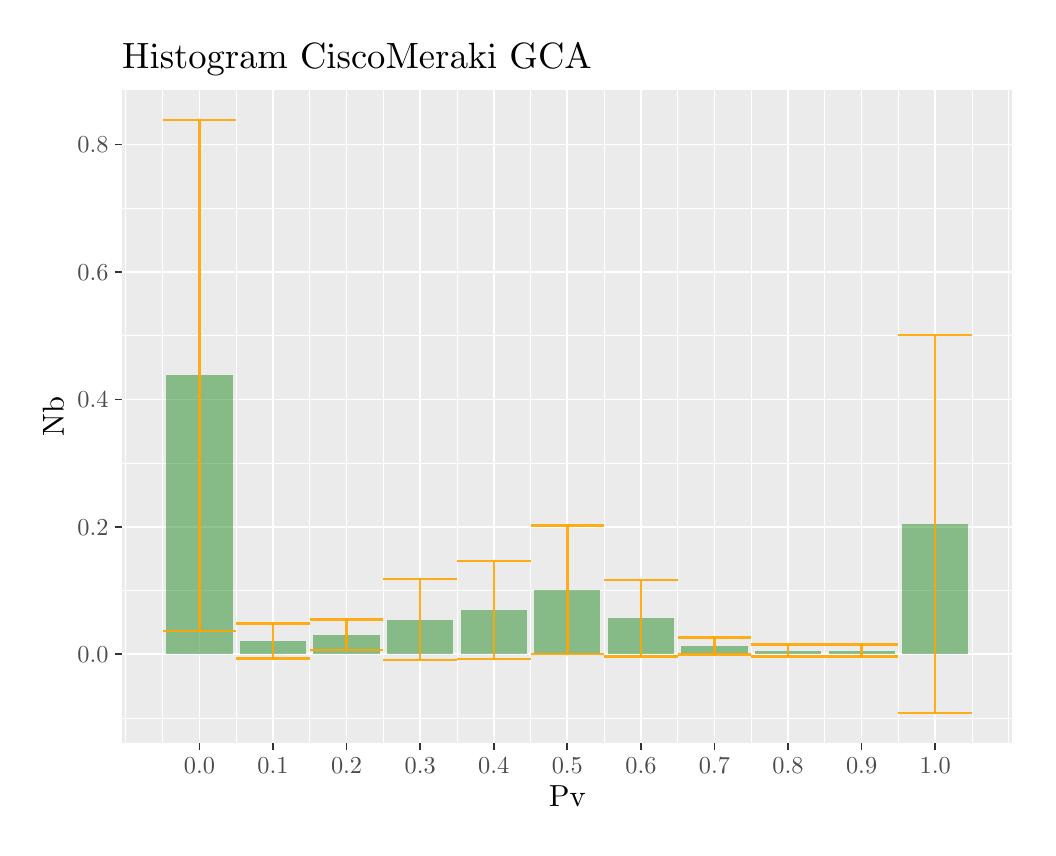
\begin{tikzpicture}[x=1pt,y=1pt]
\definecolor{fillColor}{RGB}{255,255,255}
\path[use as bounding box,fill=fillColor,fill opacity=0.00] (0,0) rectangle (361.35,289.08);
\begin{scope}
\path[clip] (  0.00,  0.00) rectangle (361.35,289.08);
\definecolor{drawColor}{RGB}{255,255,255}
\definecolor{fillColor}{RGB}{255,255,255}

\path[draw=drawColor,line width= 0.6pt,line join=round,line cap=round,fill=fillColor] (  0.00,  0.00) rectangle (361.35,289.08);
\end{scope}
\begin{scope}
\path[clip] ( 34.16, 30.69) rectangle (355.85,266.42);
\definecolor{fillColor}{gray}{0.92}

\path[fill=fillColor] ( 34.16, 30.69) rectangle (355.85,266.42);
\definecolor{drawColor}{RGB}{255,255,255}

\path[draw=drawColor,line width= 0.3pt,line join=round] ( 34.16, 39.62) --
	(355.85, 39.62);

\path[draw=drawColor,line width= 0.3pt,line join=round] ( 34.16, 85.68) --
	(355.85, 85.68);

\path[draw=drawColor,line width= 0.3pt,line join=round] ( 34.16,131.74) --
	(355.85,131.74);

\path[draw=drawColor,line width= 0.3pt,line join=round] ( 34.16,177.80) --
	(355.85,177.80);

\path[draw=drawColor,line width= 0.3pt,line join=round] ( 34.16,223.86) --
	(355.85,223.86);

\path[draw=drawColor,line width= 0.3pt,line join=round] ( 35.49, 30.69) --
	( 35.49,266.42);

\path[draw=drawColor,line width= 0.3pt,line join=round] ( 48.78, 30.69) --
	( 48.78,266.42);

\path[draw=drawColor,line width= 0.3pt,line join=round] ( 75.36, 30.69) --
	( 75.36,266.42);

\path[draw=drawColor,line width= 0.3pt,line join=round] (101.95, 30.69) --
	(101.95,266.42);

\path[draw=drawColor,line width= 0.3pt,line join=round] (128.54, 30.69) --
	(128.54,266.42);

\path[draw=drawColor,line width= 0.3pt,line join=round] (155.12, 30.69) --
	(155.12,266.42);

\path[draw=drawColor,line width= 0.3pt,line join=round] (181.71, 30.69) --
	(181.71,266.42);

\path[draw=drawColor,line width= 0.3pt,line join=round] (208.30, 30.69) --
	(208.30,266.42);

\path[draw=drawColor,line width= 0.3pt,line join=round] (234.88, 30.69) --
	(234.88,266.42);

\path[draw=drawColor,line width= 0.3pt,line join=round] (261.47, 30.69) --
	(261.47,266.42);

\path[draw=drawColor,line width= 0.3pt,line join=round] (288.06, 30.69) --
	(288.06,266.42);

\path[draw=drawColor,line width= 0.3pt,line join=round] (314.64, 30.69) --
	(314.64,266.42);

\path[draw=drawColor,line width= 0.3pt,line join=round] (341.23, 30.69) --
	(341.23,266.42);

\path[draw=drawColor,line width= 0.3pt,line join=round] (354.52, 30.69) --
	(354.52,266.42);

\path[draw=drawColor,line width= 0.6pt,line join=round] ( 34.16, 62.65) --
	(355.85, 62.65);

\path[draw=drawColor,line width= 0.6pt,line join=round] ( 34.16,108.71) --
	(355.85,108.71);

\path[draw=drawColor,line width= 0.6pt,line join=round] ( 34.16,154.77) --
	(355.85,154.77);

\path[draw=drawColor,line width= 0.6pt,line join=round] ( 34.16,200.83) --
	(355.85,200.83);

\path[draw=drawColor,line width= 0.6pt,line join=round] ( 34.16,246.89) --
	(355.85,246.89);

\path[draw=drawColor,line width= 0.6pt,line join=round] ( 62.07, 30.69) --
	( 62.07,266.42);

\path[draw=drawColor,line width= 0.6pt,line join=round] ( 88.66, 30.69) --
	( 88.66,266.42);

\path[draw=drawColor,line width= 0.6pt,line join=round] (115.24, 30.69) --
	(115.24,266.42);

\path[draw=drawColor,line width= 0.6pt,line join=round] (141.83, 30.69) --
	(141.83,266.42);

\path[draw=drawColor,line width= 0.6pt,line join=round] (168.42, 30.69) --
	(168.42,266.42);

\path[draw=drawColor,line width= 0.6pt,line join=round] (195.00, 30.69) --
	(195.00,266.42);

\path[draw=drawColor,line width= 0.6pt,line join=round] (221.59, 30.69) --
	(221.59,266.42);

\path[draw=drawColor,line width= 0.6pt,line join=round] (248.18, 30.69) --
	(248.18,266.42);

\path[draw=drawColor,line width= 0.6pt,line join=round] (274.76, 30.69) --
	(274.76,266.42);

\path[draw=drawColor,line width= 0.6pt,line join=round] (301.35, 30.69) --
	(301.35,266.42);

\path[draw=drawColor,line width= 0.6pt,line join=round] (327.93, 30.69) --
	(327.93,266.42);
\definecolor{fillColor}{RGB}{34,139,34}

\path[fill=fillColor,fill opacity=0.50] ( 50.11, 62.65) rectangle ( 74.04,163.41);

\path[fill=fillColor,fill opacity=0.50] ( 76.69, 62.65) rectangle (100.62, 67.45);

\path[fill=fillColor,fill opacity=0.50] (103.28, 62.65) rectangle (127.21, 69.73);

\path[fill=fillColor,fill opacity=0.50] (129.87, 62.65) rectangle (153.79, 75.22);

\path[fill=fillColor,fill opacity=0.50] (156.45, 62.65) rectangle (180.38, 78.64);

\path[fill=fillColor,fill opacity=0.50] (183.04, 62.65) rectangle (206.97, 85.95);

\path[fill=fillColor,fill opacity=0.50] (209.63, 62.65) rectangle (233.55, 75.67);

\path[fill=fillColor,fill opacity=0.50] (236.21, 62.65) rectangle (260.14, 65.62);

\path[fill=fillColor,fill opacity=0.50] (262.80, 62.65) rectangle (286.73, 64.02);

\path[fill=fillColor,fill opacity=0.50] (289.38, 62.65) rectangle (313.31, 64.02);

\path[fill=fillColor,fill opacity=0.50] (315.97, 62.65) rectangle (339.90,109.72);
\definecolor{drawColor}{RGB}{255,165,0}

\path[draw=drawColor,draw opacity=0.90,line width= 0.9pt,line join=round] ( 48.78,255.71) --
	( 75.36,255.71);

\path[draw=drawColor,draw opacity=0.90,line width= 0.9pt,line join=round] ( 62.07,255.71) --
	( 62.07, 71.11);

\path[draw=drawColor,draw opacity=0.90,line width= 0.9pt,line join=round] ( 48.78, 71.11) --
	( 75.36, 71.11);

\path[draw=drawColor,draw opacity=0.90,line width= 0.9pt,line join=round] ( 75.36, 73.84) --
	(101.95, 73.84);

\path[draw=drawColor,draw opacity=0.90,line width= 0.9pt,line join=round] ( 88.66, 73.84) --
	( 88.66, 61.06);

\path[draw=drawColor,draw opacity=0.90,line width= 0.9pt,line join=round] ( 75.36, 61.06) --
	(101.95, 61.06);

\path[draw=drawColor,draw opacity=0.90,line width= 0.9pt,line join=round] (101.95, 75.20) --
	(128.54, 75.20);

\path[draw=drawColor,draw opacity=0.90,line width= 0.9pt,line join=round] (115.24, 75.20) --
	(115.24, 64.26);

\path[draw=drawColor,draw opacity=0.90,line width= 0.9pt,line join=round] (101.95, 64.26) --
	(128.54, 64.26);

\path[draw=drawColor,draw opacity=0.90,line width= 0.9pt,line join=round] (128.54, 89.85) --
	(155.12, 89.85);

\path[draw=drawColor,draw opacity=0.90,line width= 0.9pt,line join=round] (141.83, 89.85) --
	(141.83, 60.59);

\path[draw=drawColor,draw opacity=0.90,line width= 0.9pt,line join=round] (128.54, 60.59) --
	(155.12, 60.59);

\path[draw=drawColor,draw opacity=0.90,line width= 0.9pt,line join=round] (155.12, 96.37) --
	(181.71, 96.37);

\path[draw=drawColor,draw opacity=0.90,line width= 0.9pt,line join=round] (168.42, 96.37) --
	(168.42, 60.92);

\path[draw=drawColor,draw opacity=0.90,line width= 0.9pt,line join=round] (155.12, 60.92) --
	(181.71, 60.92);

\path[draw=drawColor,draw opacity=0.90,line width= 0.9pt,line join=round] (181.71,109.20) --
	(208.30,109.20);

\path[draw=drawColor,draw opacity=0.90,line width= 0.9pt,line join=round] (195.00,109.20) --
	(195.00, 62.71);

\path[draw=drawColor,draw opacity=0.90,line width= 0.9pt,line join=round] (181.71, 62.71) --
	(208.30, 62.71);

\path[draw=drawColor,draw opacity=0.90,line width= 0.9pt,line join=round] (208.30, 89.55) --
	(234.88, 89.55);

\path[draw=drawColor,draw opacity=0.90,line width= 0.9pt,line join=round] (221.59, 89.55) --
	(221.59, 61.80);

\path[draw=drawColor,draw opacity=0.90,line width= 0.9pt,line join=round] (208.30, 61.80) --
	(234.88, 61.80);

\path[draw=drawColor,draw opacity=0.90,line width= 0.9pt,line join=round] (234.88, 68.74) --
	(261.47, 68.74);

\path[draw=drawColor,draw opacity=0.90,line width= 0.9pt,line join=round] (248.18, 68.74) --
	(248.18, 62.50);

\path[draw=drawColor,draw opacity=0.90,line width= 0.9pt,line join=round] (234.88, 62.50) --
	(261.47, 62.50);

\path[draw=drawColor,draw opacity=0.90,line width= 0.9pt,line join=round] (261.47, 66.26) --
	(288.06, 66.26);

\path[draw=drawColor,draw opacity=0.90,line width= 0.9pt,line join=round] (274.76, 66.26) --
	(274.76, 61.78);

\path[draw=drawColor,draw opacity=0.90,line width= 0.9pt,line join=round] (261.47, 61.78) --
	(288.06, 61.78);

\path[draw=drawColor,draw opacity=0.90,line width= 0.9pt,line join=round] (288.06, 66.26) --
	(314.64, 66.26);

\path[draw=drawColor,draw opacity=0.90,line width= 0.9pt,line join=round] (301.35, 66.26) --
	(301.35, 61.78);

\path[draw=drawColor,draw opacity=0.90,line width= 0.9pt,line join=round] (288.06, 61.78) --
	(314.64, 61.78);

\path[draw=drawColor,draw opacity=0.90,line width= 0.9pt,line join=round] (314.64,178.03) --
	(341.23,178.03);

\path[draw=drawColor,draw opacity=0.90,line width= 0.9pt,line join=round] (327.93,178.03) --
	(327.93, 41.40);

\path[draw=drawColor,draw opacity=0.90,line width= 0.9pt,line join=round] (314.64, 41.40) --
	(341.23, 41.40);
\end{scope}
\begin{scope}
\path[clip] (  0.00,  0.00) rectangle (361.35,289.08);
\definecolor{drawColor}{gray}{0.30}

\node[text=drawColor,anchor=base east,inner sep=0pt, outer sep=0pt, scale=  0.88] at ( 29.21, 59.62) {0.0};

\node[text=drawColor,anchor=base east,inner sep=0pt, outer sep=0pt, scale=  0.88] at ( 29.21,105.68) {0.2};

\node[text=drawColor,anchor=base east,inner sep=0pt, outer sep=0pt, scale=  0.88] at ( 29.21,151.74) {0.4};

\node[text=drawColor,anchor=base east,inner sep=0pt, outer sep=0pt, scale=  0.88] at ( 29.21,197.80) {0.6};

\node[text=drawColor,anchor=base east,inner sep=0pt, outer sep=0pt, scale=  0.88] at ( 29.21,243.86) {0.8};
\end{scope}
\begin{scope}
\path[clip] (  0.00,  0.00) rectangle (361.35,289.08);
\definecolor{drawColor}{gray}{0.20}

\path[draw=drawColor,line width= 0.6pt,line join=round] ( 31.41, 62.65) --
	( 34.16, 62.65);

\path[draw=drawColor,line width= 0.6pt,line join=round] ( 31.41,108.71) --
	( 34.16,108.71);

\path[draw=drawColor,line width= 0.6pt,line join=round] ( 31.41,154.77) --
	( 34.16,154.77);

\path[draw=drawColor,line width= 0.6pt,line join=round] ( 31.41,200.83) --
	( 34.16,200.83);

\path[draw=drawColor,line width= 0.6pt,line join=round] ( 31.41,246.89) --
	( 34.16,246.89);
\end{scope}
\begin{scope}
\path[clip] (  0.00,  0.00) rectangle (361.35,289.08);
\definecolor{drawColor}{gray}{0.20}

\path[draw=drawColor,line width= 0.6pt,line join=round] ( 62.07, 27.94) --
	( 62.07, 30.69);

\path[draw=drawColor,line width= 0.6pt,line join=round] ( 88.66, 27.94) --
	( 88.66, 30.69);

\path[draw=drawColor,line width= 0.6pt,line join=round] (115.24, 27.94) --
	(115.24, 30.69);

\path[draw=drawColor,line width= 0.6pt,line join=round] (141.83, 27.94) --
	(141.83, 30.69);

\path[draw=drawColor,line width= 0.6pt,line join=round] (168.42, 27.94) --
	(168.42, 30.69);

\path[draw=drawColor,line width= 0.6pt,line join=round] (195.00, 27.94) --
	(195.00, 30.69);

\path[draw=drawColor,line width= 0.6pt,line join=round] (221.59, 27.94) --
	(221.59, 30.69);

\path[draw=drawColor,line width= 0.6pt,line join=round] (248.18, 27.94) --
	(248.18, 30.69);

\path[draw=drawColor,line width= 0.6pt,line join=round] (274.76, 27.94) --
	(274.76, 30.69);

\path[draw=drawColor,line width= 0.6pt,line join=round] (301.35, 27.94) --
	(301.35, 30.69);

\path[draw=drawColor,line width= 0.6pt,line join=round] (327.93, 27.94) --
	(327.93, 30.69);
\end{scope}
\begin{scope}
\path[clip] (  0.00,  0.00) rectangle (361.35,289.08);
\definecolor{drawColor}{gray}{0.30}

\node[text=drawColor,anchor=base,inner sep=0pt, outer sep=0pt, scale=  0.88] at ( 62.07, 19.68) {0.0};

\node[text=drawColor,anchor=base,inner sep=0pt, outer sep=0pt, scale=  0.88] at ( 88.66, 19.68) {0.1};

\node[text=drawColor,anchor=base,inner sep=0pt, outer sep=0pt, scale=  0.88] at (115.24, 19.68) {0.2};

\node[text=drawColor,anchor=base,inner sep=0pt, outer sep=0pt, scale=  0.88] at (141.83, 19.68) {0.3};

\node[text=drawColor,anchor=base,inner sep=0pt, outer sep=0pt, scale=  0.88] at (168.42, 19.68) {0.4};

\node[text=drawColor,anchor=base,inner sep=0pt, outer sep=0pt, scale=  0.88] at (195.00, 19.68) {0.5};

\node[text=drawColor,anchor=base,inner sep=0pt, outer sep=0pt, scale=  0.88] at (221.59, 19.68) {0.6};

\node[text=drawColor,anchor=base,inner sep=0pt, outer sep=0pt, scale=  0.88] at (248.18, 19.68) {0.7};

\node[text=drawColor,anchor=base,inner sep=0pt, outer sep=0pt, scale=  0.88] at (274.76, 19.68) {0.8};

\node[text=drawColor,anchor=base,inner sep=0pt, outer sep=0pt, scale=  0.88] at (301.35, 19.68) {0.9};

\node[text=drawColor,anchor=base,inner sep=0pt, outer sep=0pt, scale=  0.88] at (327.93, 19.68) {1.0};
\end{scope}
\begin{scope}
\path[clip] (  0.00,  0.00) rectangle (361.35,289.08);
\definecolor{drawColor}{RGB}{0,0,0}

\node[text=drawColor,anchor=base,inner sep=0pt, outer sep=0pt, scale=  1.10] at (195.00,  7.64) {Pv};
\end{scope}
\begin{scope}
\path[clip] (  0.00,  0.00) rectangle (361.35,289.08);
\definecolor{drawColor}{RGB}{0,0,0}

\node[text=drawColor,rotate= 90.00,anchor=base,inner sep=0pt, outer sep=0pt, scale=  1.10] at ( 13.08,148.55) {Nb};
\end{scope}
\begin{scope}
\path[clip] (  0.00,  0.00) rectangle (361.35,289.08);
\definecolor{drawColor}{RGB}{0,0,0}

\node[text=drawColor,anchor=base west,inner sep=0pt, outer sep=0pt, scale=  1.32] at ( 34.16,274.49) {Histogram CiscoMeraki GCA};
\end{scope}
\end{tikzpicture}
